\subsection{ADEQUATE}
\label{subsec:noah__adequate}

The final `new' module to be described in this section is the 1,1-ADEQUATE experiment\autocite{Reif1996JMRSA}, which provides two-bond \ch{C}--\ch{H} correlations through a combination of $\oneJ{CH}$ and $\oneJ{CC}$.
Because of the requirement for two adjacent \carbon{} nuclei, the sensitivity of the ADEQUATE experiment is considerably lower than almost all other NOAH modules considered so far.
As established in \cref{subsec:noah__snr}, sensitivity imbalances between different modules lead to less ideal supersequences with smaller effective time savings $\rho_{t,\text{eff}}$.
Thus, the ADEQUATE module has to date not been implemented in NOAH supersequences.%
\footnote{There is, in fact, one exception to my claim\autocite{RaoKakita2020RSCA}. Here, the ADEQUATE and seHSQC modules were not modified to preserve any magnetisation for later modules. Since the ADEQUATE itself has such low sensitivity, it is likely that the sensitivity losses in the later modules were tolerable; however, no sensitivity comparisons against standalone experiments were provided.}

In this section, I only consider the design of the NOAH ADEQUATE module itself, which turns out to be extraordinarily simple.
The \proton{} pulses in the original ADEQUATE experiment mirror that of the CRK seHSQC almost perfectly, save for one extra \ang{180} pulse.
In particular, the INEPT excitation and the PEP transfer element are the same.
Thus, the ADEQUATE module can be modified to preserve \magnnot{C} magnetisation using exactly the same strategy in seHSQC2: namely, replacing the first \proton{} excitation pulse with the ZIP element (\cref{fig:adequate_noah}).
In order to compensate for the extra \ang{180} pulse (which arises in the constant-time period), the pulse phases in the ZIP element are modified accordingly: thus, the third \proton{} \ang{90} pulse has a phase of $y\/$ (instead of $-y\/$ in seHSQC2).

\begin{figure}[htb]
    \centering
    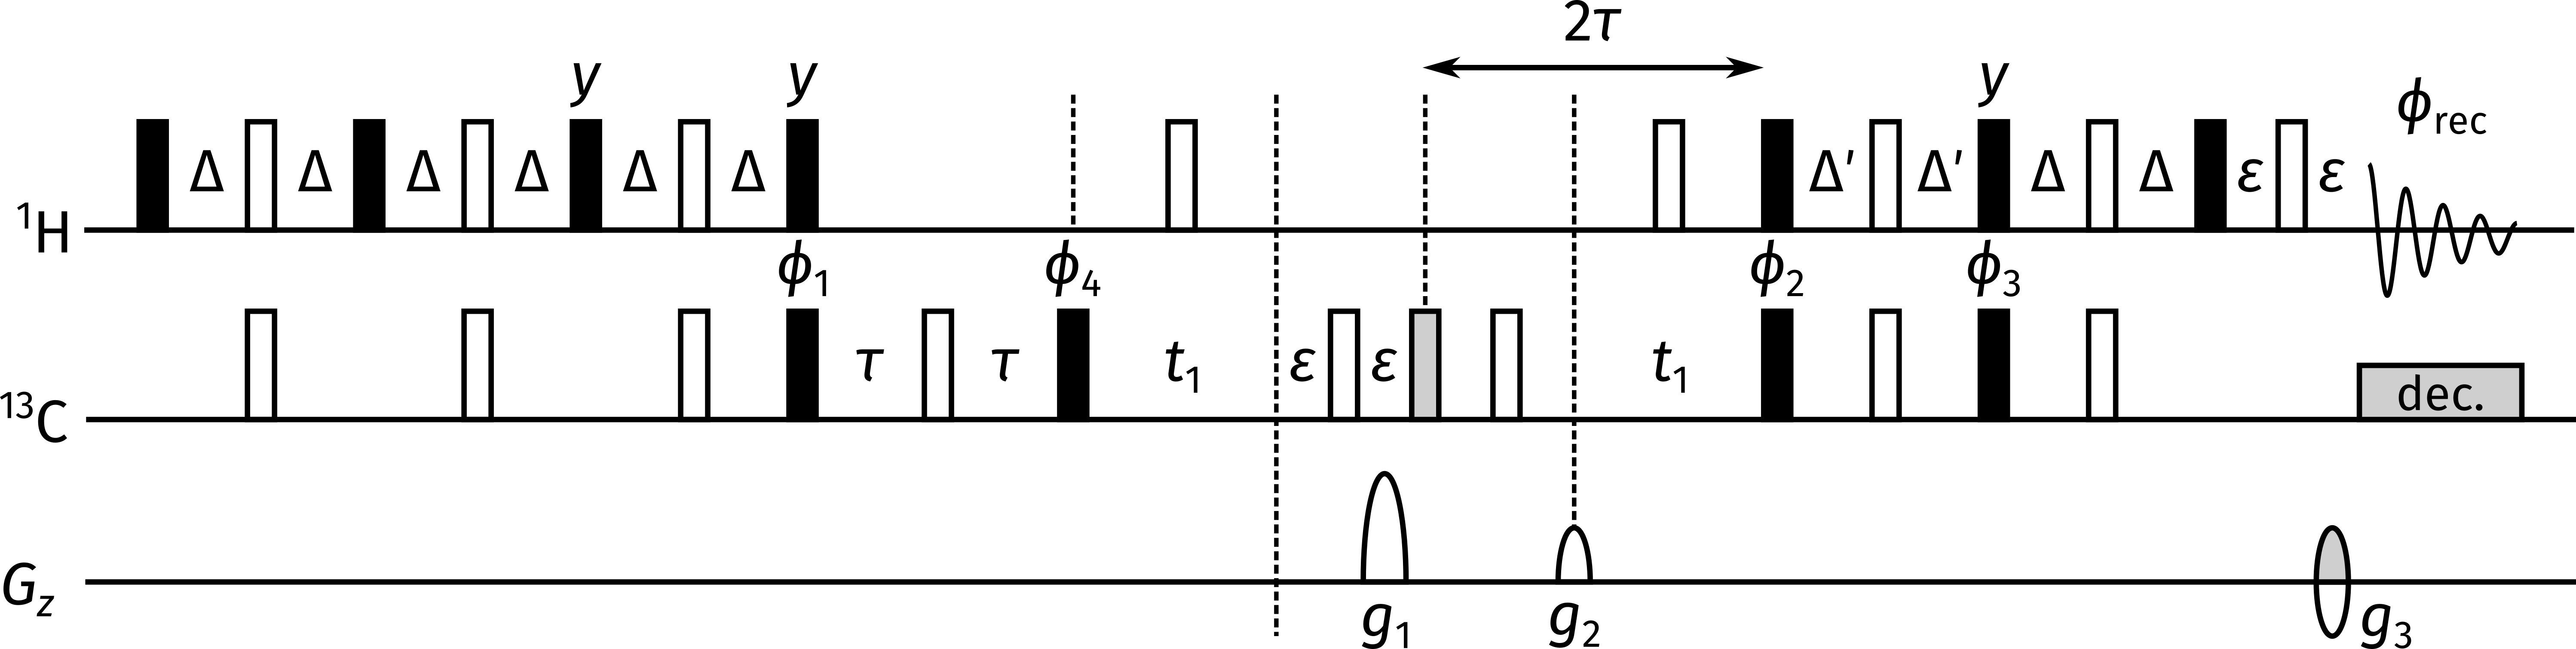
\includegraphics[]{pp/adequate.png}%
    \caption[NOAH 1,1-ADEQUATE module]{
        NOAH 1,1-ADEQUATE module.
        The grey filled bar is a \ang{120} pulse, optimised for \carbon{} double-quantum to single-quantum coherence transfer\autocite{Mareci1982JMR}.
        Delays are set as follows: $\Delta = 1 / (4 \cdot \oneJ{CH})$, $\Delta' = 1 / (8 \cdot \oneJ{CH})$, and $\tau = 1 / (4 \cdot \oneJ{CC})$.
        Phase cycling is performed using $\phi_1 = (x, -x)$, $\phi_2 = (x, x, -x, -x)$, $\phi_3 = (y, y, -y, -y)$, $\phi_4 = (x, x, x, x, -x, -x, -x, -x)$, and $\phi_\text{rec} = (x, -x, -x, x, -x, x, x, -x)$.
        Gradient amplitudes are $(g_1, g_2, g_3) = (78.5\%, 77.6\%, \mp 59\%)$.
        Echo--antiecho selection is achieved by inverting the sign of $g_3$ as well as the pulse phase $\phi_3$.
    }
    \label{fig:adequate_noah}
\end{figure}

An example of a \noah{A,B} supersequence is shown in \cref{fig:noah_ab}.
This is not the best setting to use the ADEQUATE module in, because the \carbon{} HMBC module has roughly 100 times the sensitivity of the ADEQUATE; however, it demonstrates that the ADEQUATE module does indeed work as intended.
More constructive uses of the ADEQUATE module are deferred to \cref{sec:noah__parallel}: in there, I discuss combinations with the (lower-sensitivity) \nitrogen{} HMBC module, and show how other modules may be added to form so-called `generalised' supersequences.

\begin{figure}[htb]
    \centering
    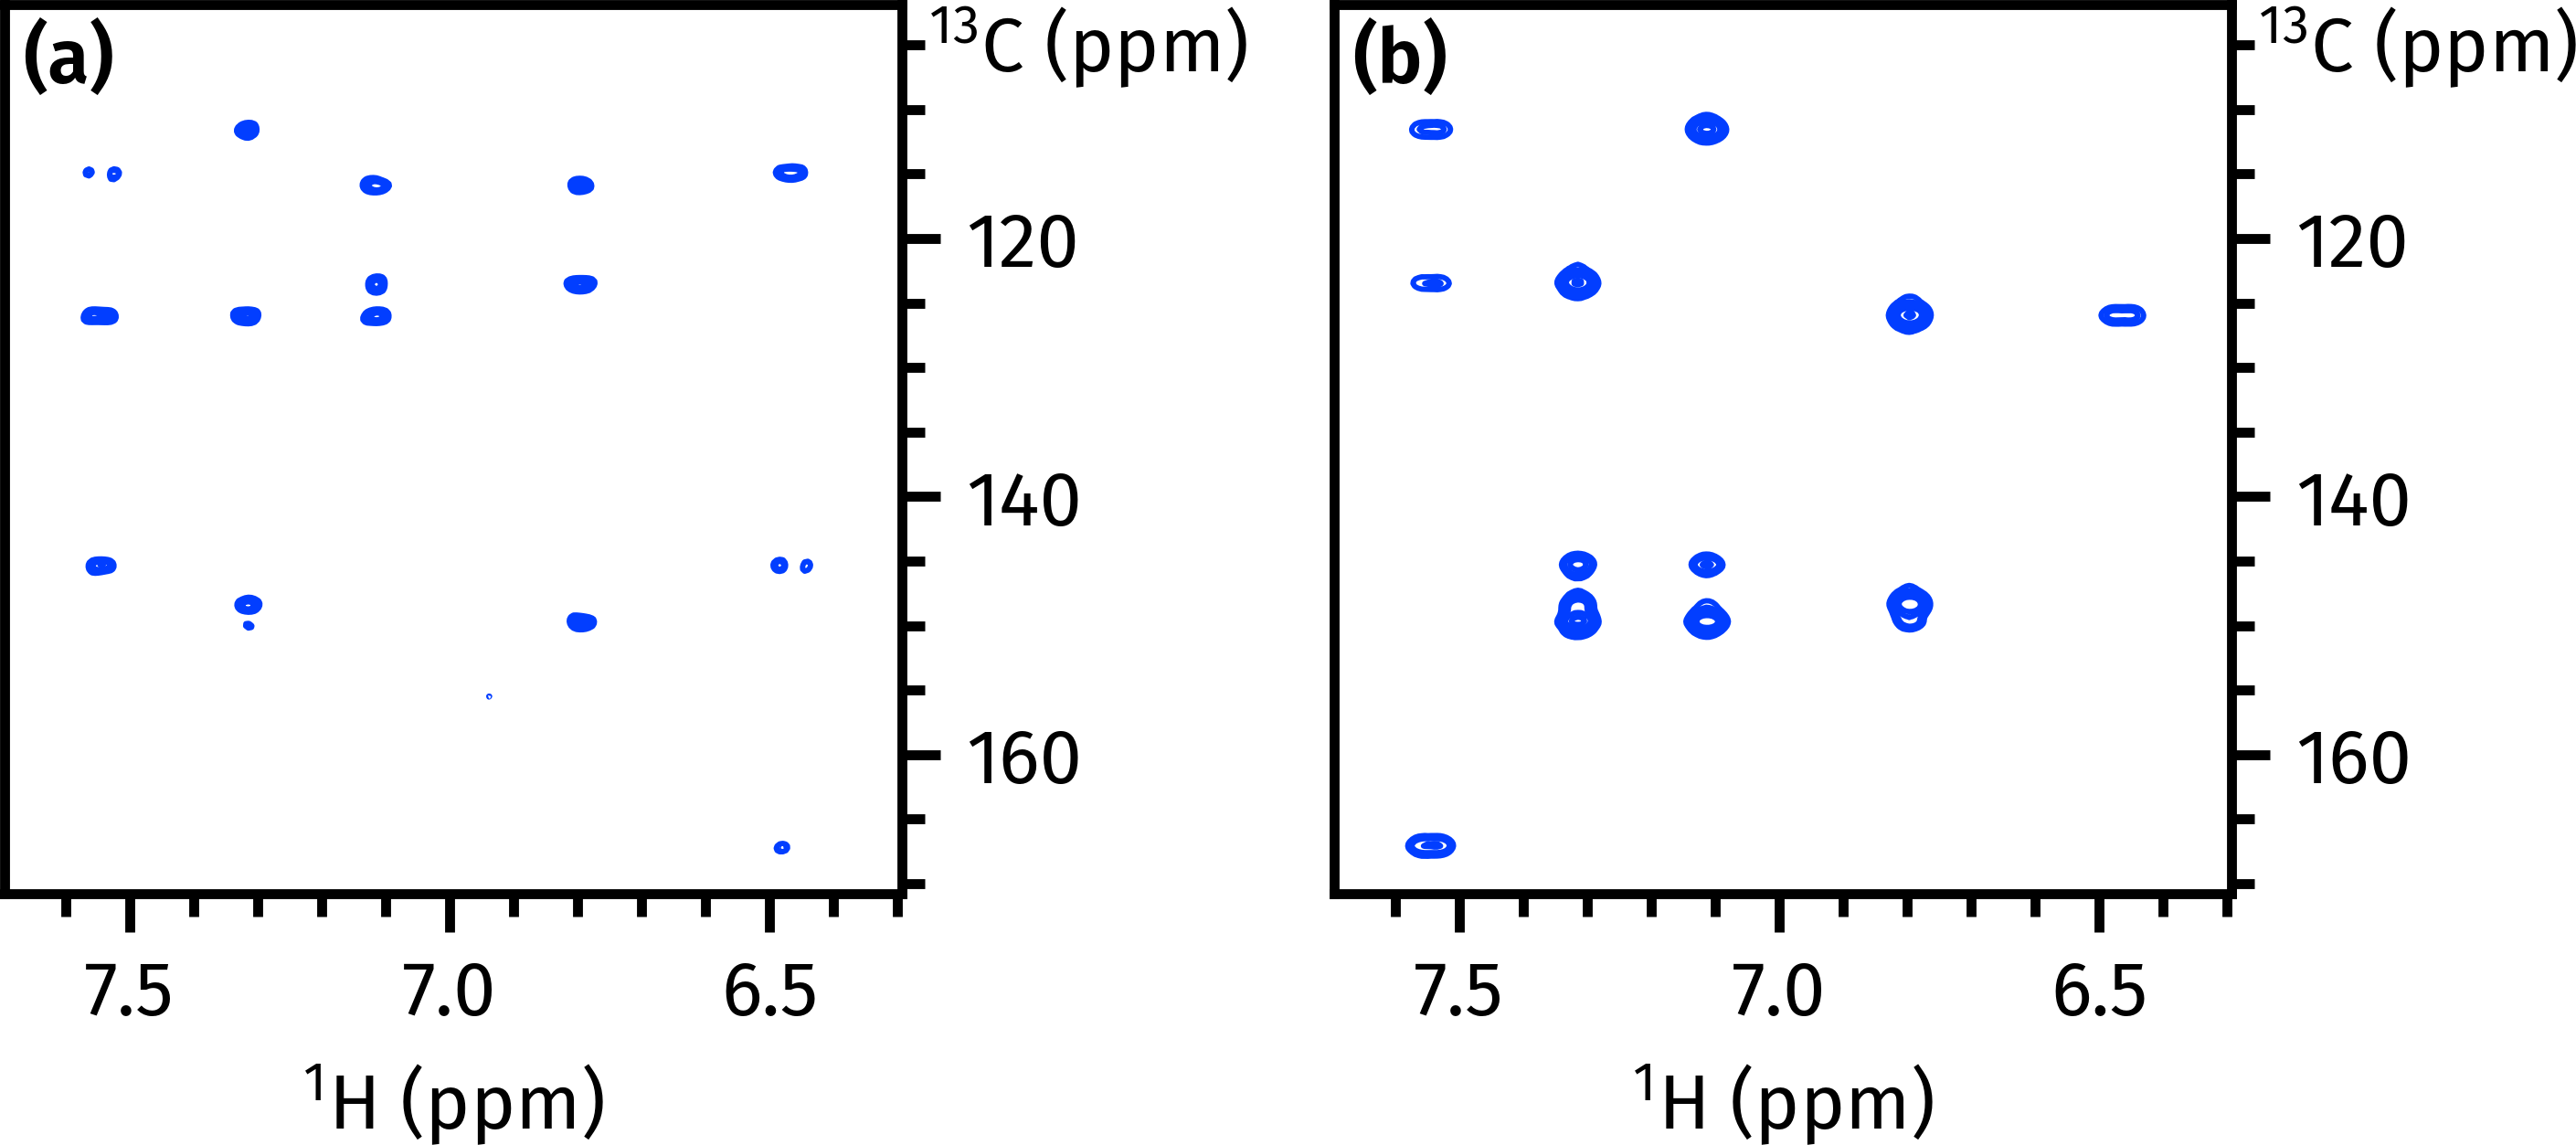
\includegraphics[]{noah/ab.png}%
    {\phantomsubcaption\label{fig:noah_ab_a}}%
    \caption[Spectra from \noah{A,B} supersequence]{
        Spectra from a \noah{A,B} supersequence.
        \textbf{(\subref*{fig:noah_ab_a})} 1,1-ADEQUATE module.
        \textbf{(\subref*{fig:noah_ab_a})} HMBC module.
        \datacode{7T-211231}
    }
    \label{fig:noah_ab}
\end{figure}
